\documentclass{article}

% Language setting
% Replace `english' with e.g. `spanish' to change the document language
\usepackage[english]{babel}

% Set page size and margins
% Replace `letterpaper' with `a4paper' for UK/EU standard size
\usepackage[letterpaper,top=2cm,bottom=2cm,left=3cm,right=3cm,marginparwidth=1.75cm]{geometry}

% Useful packages
\usepackage{amsmath}
\usepackage{graphicx}
\usepackage{appendix}
\usepackage[colorlinks=true, allcolors=blue]{hyperref}
\usepackage{caption}
\captionsetup{justification=centering}

\title{Airframe Optimization}
\author{Ryan Howell}

\begin{document}
\maketitle

%\begin{abstract}

%\end{abstract}

\section{Introduction}

Through reading the textbook and SNOW.jl documentation as part of this assignment, I learned about optimization processes and how to set up optimization problems using SNOW.jl. By experimenting with SNOW.jl inputs, I observed the aerodynamic effects of wing shape, twist, and angle of attack particularly when optimizing for drag. In this report, I will discuss some key takeaways from the readings and explore the optimization process and resulting wings when varying specific parameters. These results will be explained using theory and analytical results from previous projects.

\section{Background Readings}
The suggested readings included a basic overview of the design process, with a focus on the role of optimization. They also covered the required setup to use the SNOW.jl optimization wrapper and its capabilities.

\subsection{Design Process}
The design process requires that an initial design be set, then evaluated, modified, and iterated until a good or optimal design is achieved. With an optimization algorithm, this iterative design can be repeated more quickly and find a better solution in most cases than repeated hand calculations. However, it requires the optimization problem to be formulated and set up with constraints, an optimized parameter, and input variables. 

\subsection{SNOW.jl}
To optimize in the SNOW.jl wrapper, the number of constraints must be set with upper and lower bounds, typically negative infinity to zero. The constraints are then defined in the function being optimized. The input parameters for the function also need to be defined with a range of potential values and an initial starting value. Once these are done, the minimize function can be called to optimize the design parameters for the given objective.

\section{Optimized Airframe Design}
Building on the airframe analysis of the previous report, I used the Vortex Lattice method to set up an optimization problem to find the best wing shape.

\subsection{Chord Distribution}
The primary objective of this project was to optimize the chord distribution of a wing. This is accomplished by using the vortex lattice method to approximate the lift and drag of a wing in a function that was then optimized with the SNOW.jl wrapper. The objective was to minimize drag and maintain a required lift of 1.7 pounds, with constraints ensuring the wings retain a reasonable shape. These constraints include ensuring the chord length decreases across the span of the wing and limiting the variation between sections to a reasonable amount based on the number of sections. This approach maintains a realistic wing that meets the operating conditions for the plane while reducing the drag on the wing, or the required thrust.

\subsubsection{Changing the Number of Sections}
Changing the number of sections allowed for increased refinement, as seen by comparing Figures \ref{fig:Low Res} and \ref{fig:High Res}. This creates a more accurate representation of the optimized wing. However, too many sections significantly slow down the optimization without much added resolution. In the refined wing profile, the optimized planform area is very elliptical, with the main deviation at the tip where it ends abruptly flat. This design avoids the sharp increase in lift coefficient predicted by Vortex Lattice for wings with sharp tips, as shown in the project 2 report.

\begin{figure}[h]
\centering
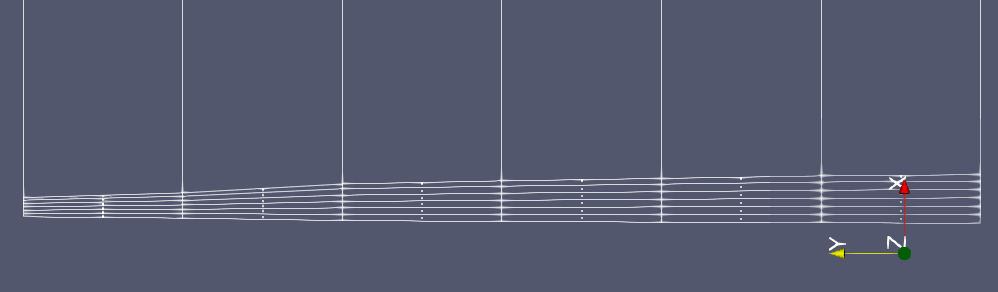
\includegraphics[width=\textwidth]{LOW RES FOCUSED.png}
\caption{Optimized wing of 6 sections}
\label{fig:Low Res}
\end{figure}

\begin{figure}[h]
\centering
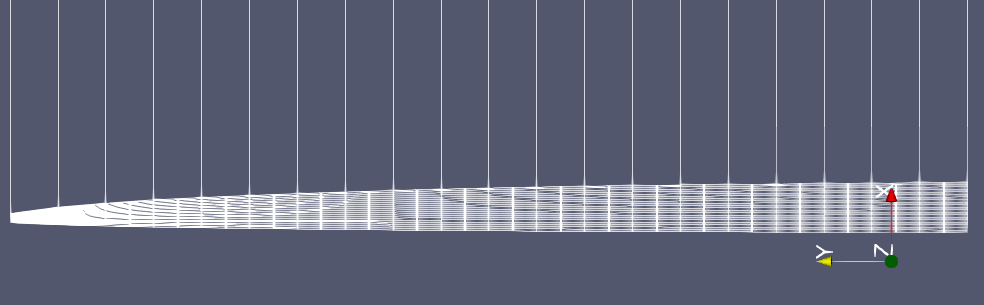
\includegraphics[width=\textwidth]{HIGH RES FOCUSED.png}
\caption{Optimized wing of 20 sections}
\label{fig:High Res}
\end{figure}

\subsection{The Effect of Constraints}
Upon finding the optimal wing chord distribution, the restrictions on the change in chord from one section to the next were removed, leaving only the lift restriction. Using the previously found chord distribution as the initial starting point, it converged to the same solution, shown in Figure \ref{fig:High Res}, confirming its optimality and the appropriateness of those constraints. Then I varied the lift constraint by changing the weight of the aircraft, which had a drastic effect on the wing lift distribution. As seen in Figure \ref{fig:Slightly Higher}, adding 4 pounds to the lift constraint caused the wing chords to lengthen. Increasing the lift constraint by a factor of five lengthened the chords even more, see Figure \ref{fig:5 Higher}. This adjustment creates more lift while maintaining an elliptical shape. These larger wings resemble those of a Supermarine Spitfire, with the main difference being at the wingtips due to Vortex Lattice limitations as previously discussed. Increasing the plane's weight also increased the time needed to optimize the problem.

\begin{figure}[h]
    \centering
\begin{minipage}[b]{0.45\textwidth}
\centering
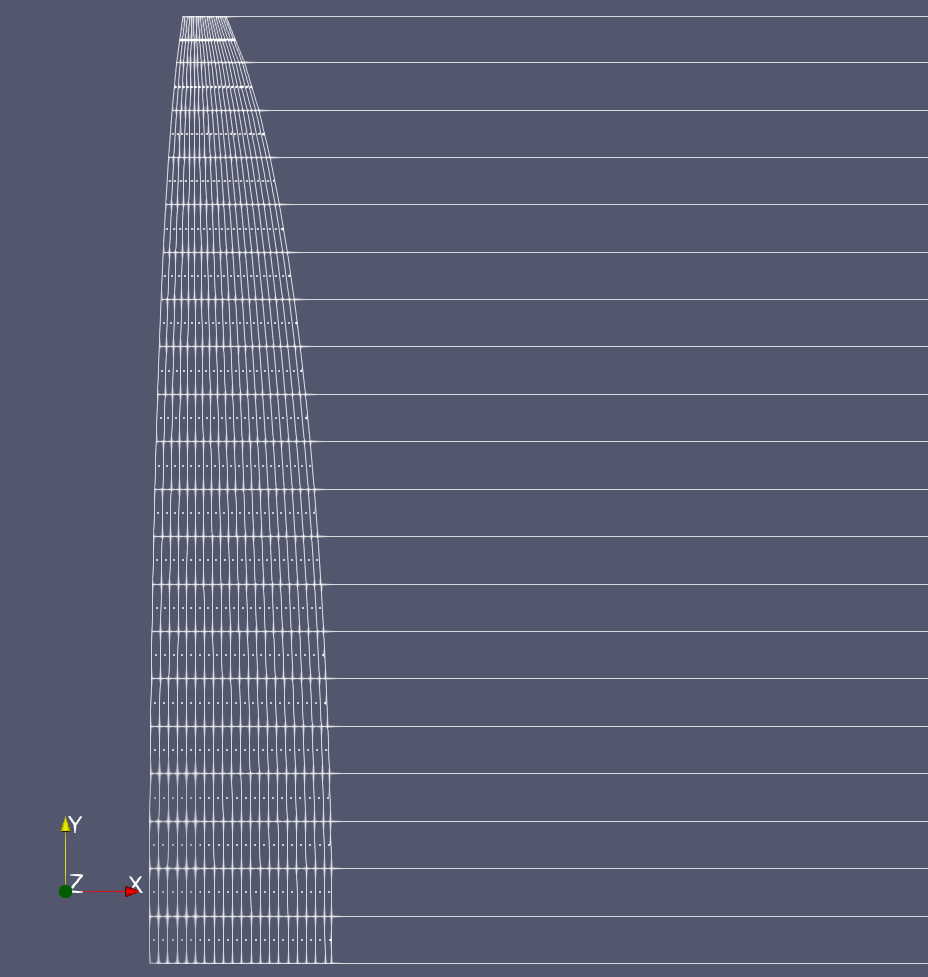
\includegraphics[width=\textwidth]{4 pounds more.png}
\caption{Optimized wing with 4 additional pounds}
\label{fig:Slightly Higher}
\end{minipage}
\begin{minipage}[b]{0.45\textwidth}
\centering
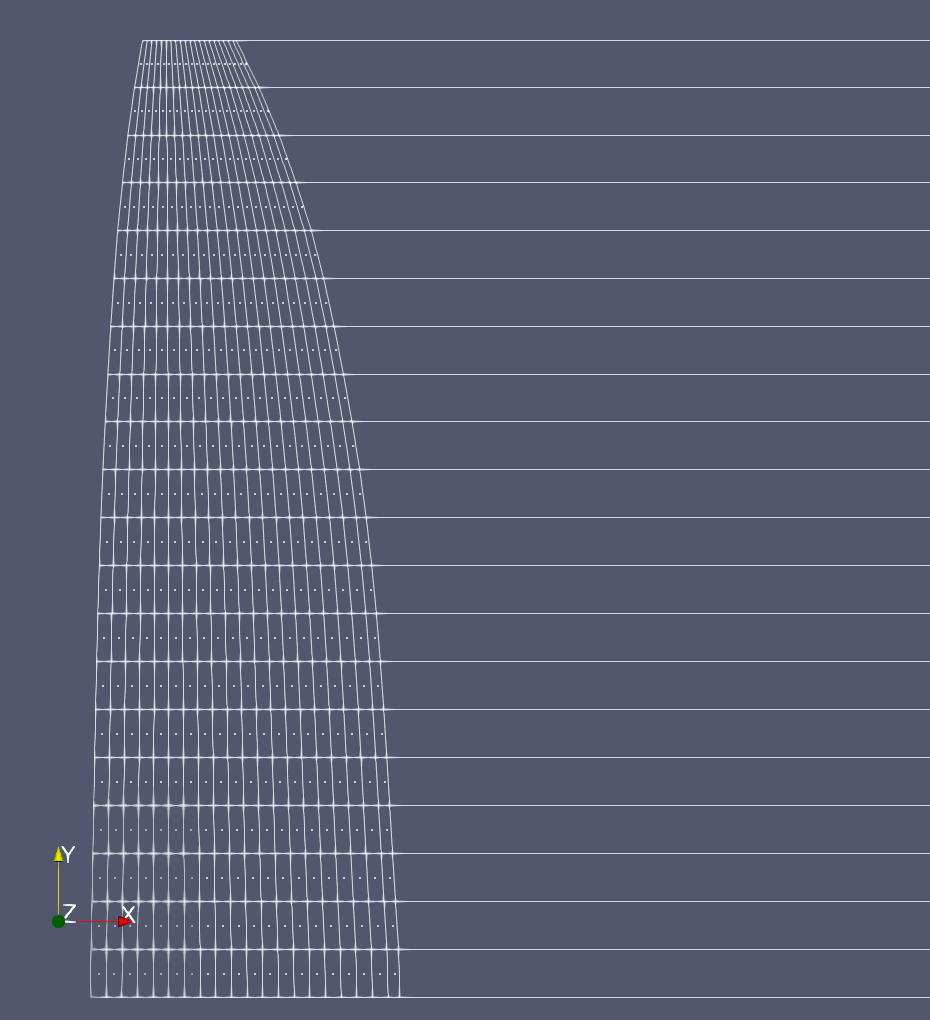
\includegraphics[width=\textwidth]{5 Times load.png}
\caption{Optimized wing with 5 times the load}
\label{fig:5 Higher}
\end{minipage}
\end{figure}

\subsection{The Effect of the Tolerance}

Increasing the lift constraint eventually leads to unsolvable scenarios, resulting in square wings or, through repeated iterations, partially square and elliptic wings but never converging to a solution. This can be reduced by increasing the tolerance, allowing the optimizer to run more quickly and reduce the precision of its search. Using the optimized chord distribution from previous iterations as an initial point, you can decrease the tolerance until an adequate tolerance is achieved. This approach allows for the wing to be optimized at a high tolerance for a more extreme scenario.

\section{Different Optimization Problems}

To deepen my familiarity with optimization problems and the SNOW.jl wrapper, I completed two additional optimization problems from the appendix of the handout. The first problem added a second variable to optimize: the angle of attack or pitch. The second problem optimized the twist of the wing while holding the chord and pitch constant.

\subsection{Optimizing Pitch Along with Chord Distribution}
In this optimization problem, I had to pass in all the variables as one vector, which required separating the chords from the alpha value in the function. Once done, I could optimize the chord distribution and alpha angle separately. Interestingly, as shown in Figures \ref{fig:Optimized Alpha Small Load} and \ref{fig:Optimized Alpha Large Load}, the root chord varied significantly less under increased loading. The angle of attack was optimized to produce more lift while minimizing drag further. This led to a larger root chord at the normal lift requirement, 1.7 pounds, and a smaller root chord at 5 times that lift requirement. Comparing Figures \ref{fig:Optimized Alpha Small Load} and \ref{fig:Optimized Alpha Large Load} with Figures \ref{fig:High Res} and \ref{fig:5 Higher}  highlights these differences. As noted in the image captions, the angle of attack increases with weight, which intuitively makes sense as a higher angle of attack produces more lift while adding some drag. The Vortex Lattice method introduces some inaccuracies at high alpha angles of attack as it doesn't account for stall. This was minimized by setting up the optimizer problem with a max alpha of around 15 degrees, which is near the stall angle of most airfoils.

\begin{figure}[h]
    \centering
\begin{minipage}[b]{0.45\textwidth}
\centering
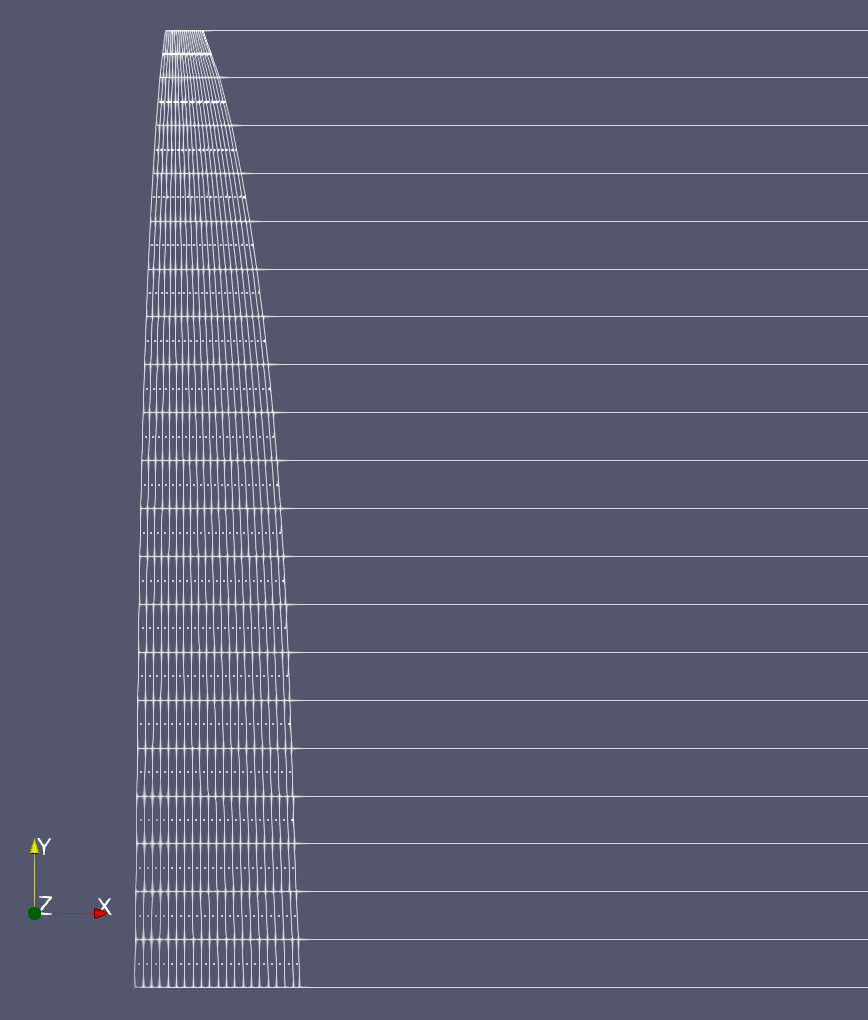
\includegraphics[width=\textwidth]{1 scale optimized alpha.png}
\caption{Optimized wing for base lift constraint and an optimized alpha of about 1.7 degrees}
\label{fig:Optimized Alpha Small Load}
\end{minipage}
\begin{minipage}[b]{0.45\textwidth}
\centering
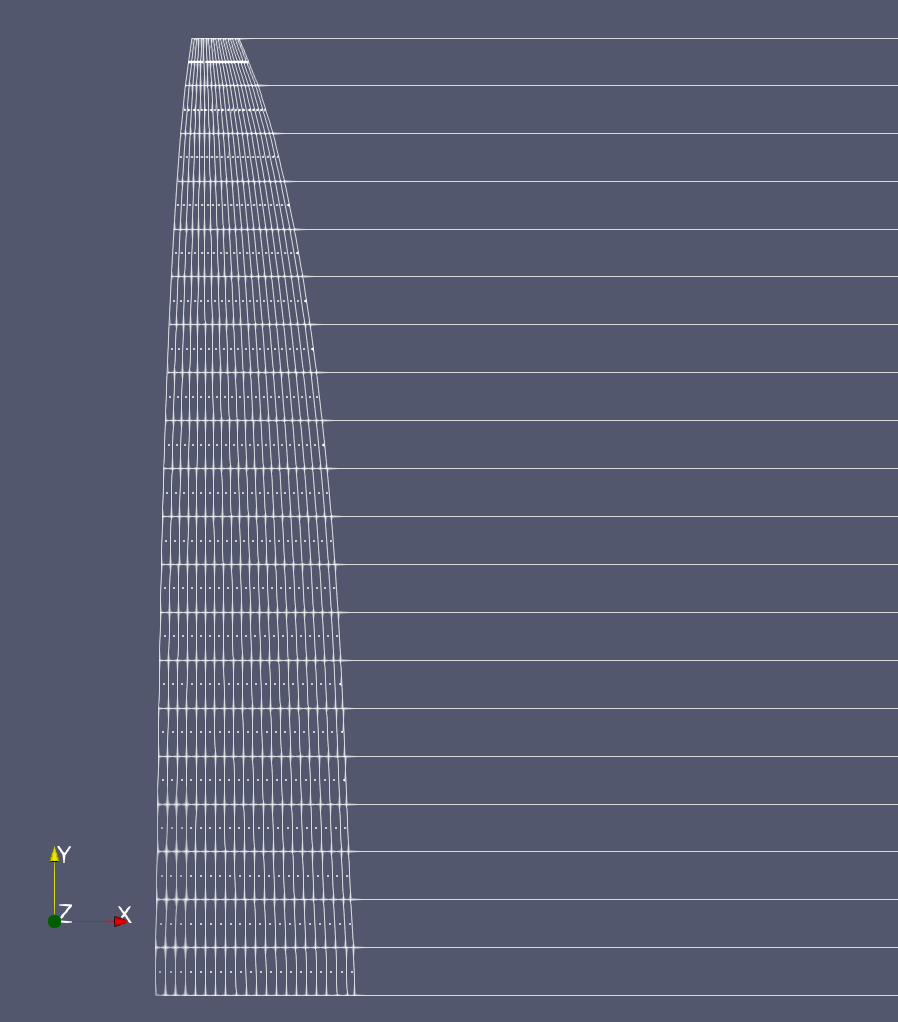
\includegraphics[width=\textwidth]{5 scale optimized alpha.png}
\caption{Optimized wing with 5 times the load and an optimized alpha of about 7.2 degrees}
\label{fig:Optimized Alpha Large Load}
\end{minipage}
\end{figure}

\subsection{Varying Twist Angle}
In this study, the chord distribution was kept constant across the wing span. The optimizer adjusted the theta vector to minimize drag while maintaining the required lift, allowing for negative twist. This optimization resulted in an elliptical lift distribution, as shown in Figures \ref{fig:Optimized Twist Small Load} and \ref{fig:Optimized Twist Large Load}.  The figures demonstrate that increasing the plane's weight causes the optimizer to generate more lift through additional twist while maintaining an elliptical lift distribution. This was done by increasing the twist of the wing. This indicates that wing twist can yield the same optimal lift distribution as an elliptical wing with other wing shapes. 

\begin{figure}[h]
    \centering
\begin{minipage}[b]{0.45\textwidth}
\centering
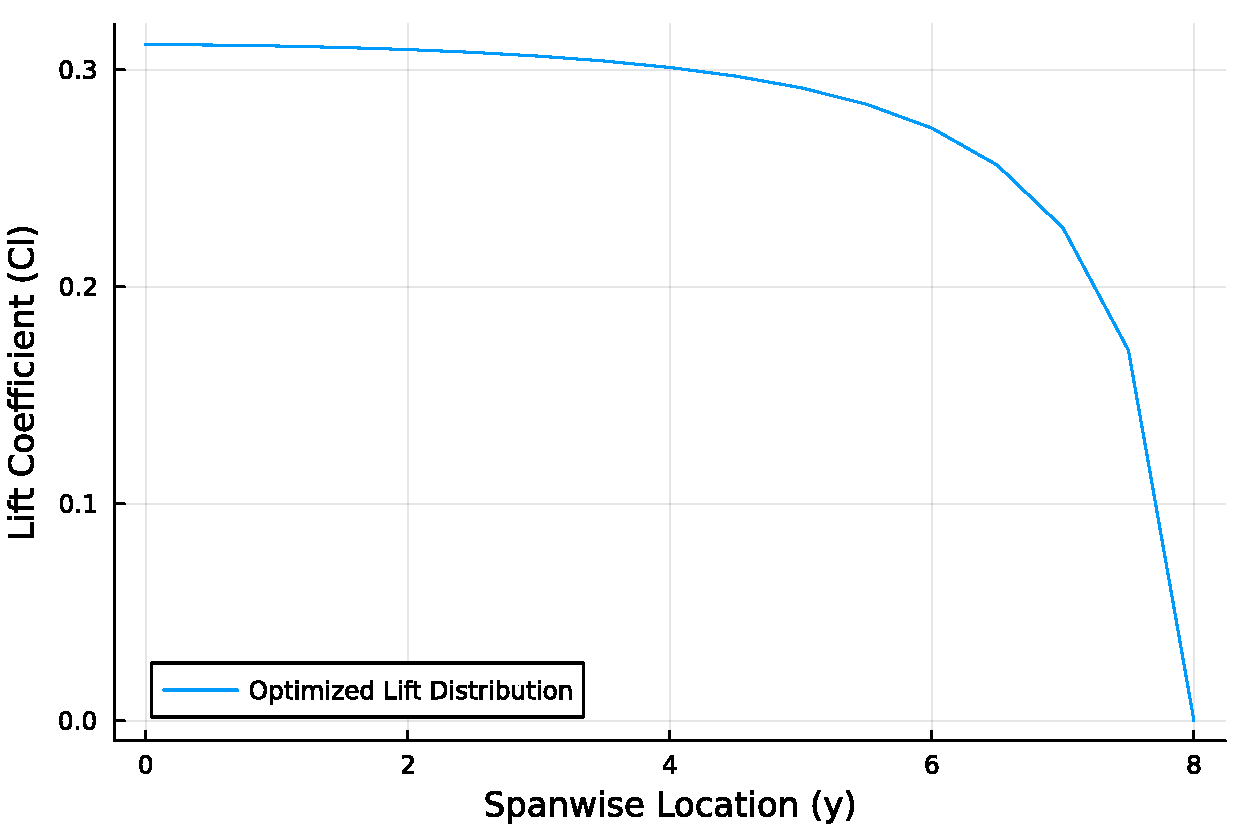
\includegraphics[width=\textwidth]{Lift_Distribution_along_the_Span_Twist_Optimization.pdf}
\caption{Lift distribution of a twisted, rectangular wing}
\label{fig:Optimized Twist Small Load}
\end{minipage}
\begin{minipage}[b]{0.45\textwidth}
\centering
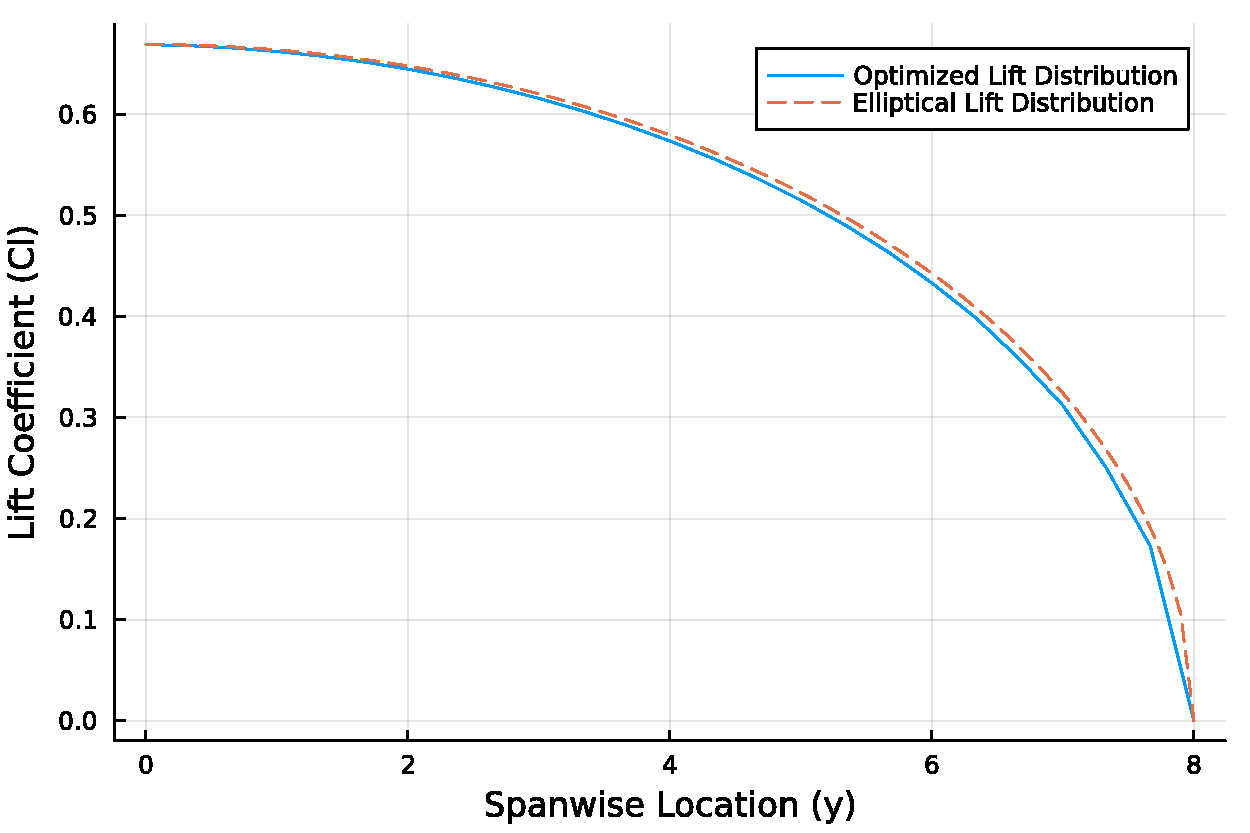
\includegraphics[width=\textwidth]{Lift_Distribution_along_the_Span_Twist_Optimization_increased_lift.pdf}
\caption{Lift distribution of a twisted, rectangular wing with increased weight}
\label{fig:Optimized Twist Large Load}
\end{minipage}
\end{figure}

\section{Conclusion}
This project provided a solid understanding of optimization processes through readings and the implementation of aerodynamic optimization problems in SNOW.jl. By experimenting with parameters such as wing shape, twist, and angle of attack, I gained insights into airframe design and the formulation of various optimization problems. The optimized solutions aligned intuitively with analytical results and theory from previous projects. Overall, this project deepened my theoretical knowledge and offered practical experience in solving optimization problems, highlighting the advantages of optimization tools in aerospace engineering.


%\bibliographystyle{alpha}
%\bibliography{sample}

%\clearpage
%\appendix
%\chapter{Appendix A}

\end{document}